\documentclass{article}
% Change "article" to "report" to get rid of page number on title page
\usepackage{amsmath,amsfonts,amsthm,amssymb}
\usepackage{setspace}
\usepackage{fancyhdr}
\usepackage{lastpage}
\usepackage{extramarks}
\usepackage{chngpage}
\usepackage{soul}
\usepackage[usenames,dvipsnames]{color}
\usepackage{graphicx,float,wrapfig}
\usepackage{ifthen}
\usepackage{listings}
\usepackage{courier}


%   !!!!!!!!!!!!!!!!!!!!!!!!!!!!!!!!!!!!!!!!!!!!!!!!!!!!!
%
%   Here put your info (name, due date, title etc).
%   the rest should be left unchanged.
%
%
%
%   !!!!!!!!!!!!!!!!!!!!!!!!!!!!!!!!!!!!!!!!!!!!!!!!!!!!!


% Homework Specific Information
\newcommand{\hmwkTitle}{}
\newcommand{\hmwkSubTitle}{Fourier transforms and analysis}
\newcommand{\hmwkDueDate}{March 30, 2023}
\newcommand{\hmwkClass}{Computational Physics III}
\newcommand{\hmwkClassTime}{}
%\newcommand{\hmwkClassInstructor}{Prof. Oleg Yazyev}
\newcommand{\hmwkAuthorName}{Salomon Guinchard}
\newcommand{\beq}{\begin{equation}}
\newcommand{\eeq}{\end{equation}}
\graphicspath{{./Illustrations/}{./IllustrationsResults/}}  
%
%


% In case you need to adjust margins:
\topmargin=-0.45in      %
\evensidemargin=0in     %
\oddsidemargin=0in      %
\textwidth=6.5in        %
\textheight=9.5in       %
\headsep=0.25in         %

% This is the color used for  comments below
\definecolor{MyDarkGreen}{rgb}{0.0,0.4,0.0}

% For faster processing, load Matlab syntax for listings
\lstloadlanguages{Matlab}%
\lstset{language=Matlab,                        % Use MATLAB
        frame=single,                           % Single frame around code
        basicstyle=\small\ttfamily,             % Use small true type font
        keywordstyle=[1]\color{Blue}\bf,        % MATLAB functions bold and blue
        keywordstyle=[2]\color{Purple},         % MATLAB function arguments purple
        keywordstyle=[3]\color{Blue}\underbar,  % User functions underlined and blue
        identifierstyle=,                       % Nothing special about identifiers
                                                % Comments small dark green courier
        commentstyle=\usefont{T1}{pcr}{m}{sl}\color{MyDarkGreen}\small,
        stringstyle=\color{Purple},             % Strings are purple
        showstringspaces=false,                 % Don't put marks in string spaces
        tabsize=3,                              % 5 spaces per tab
        %
        %%% Put standard MATLAB functions not included in the default
        %%% language here
        morekeywords={xlim,ylim,var,alpha,factorial,poissrnd,normpdf,normcdf},
        %
        %%% Put MATLAB function parameters here
        morekeywords=[2]{on, off, interp},
        %
        %%% Put user defined functions here
        morekeywords=[3]{FindESS, homework_example},
        %
        morecomment=[l][\color{Blue}]{...},     % Line continuation (...) like blue comment
        numbers=left,                           % Line numbers on left
        firstnumber=1,                          % Line numbers start with line 1
        numberstyle=\tiny\color{Blue},          % Line numbers are blue
        stepnumber=1                        % Line numbers go in steps of 5
        }

% Setup the header and footer
\pagestyle{fancy}                                                       %
\lhead{\hmwkAuthorName}                                                 %
%\chead{\hmwkClass\ (\hmwkClassInstructor\ \hmwkClassTime): \hmwkTitle}  %
\rhead{\hmwkClass\ : \hmwkTitle}  %
%\rhead{\firstxmark}                                                     %
\lfoot{\lastxmark}                                                      %
\cfoot{}                                                                %
\rfoot{Page\ \thepage\ of\ \protect\pageref{LastPage}}                  %
\renewcommand\headrulewidth{0.4pt}                                      %
\renewcommand\footrulewidth{0.4pt}                                      %

% This is used to trace down (pin point) problems
% in latexing a document:
%\tracingall

%%%%%%%%%%%%%%%%%%%%%%%%%%%%%%%%%%%%%%%%%%%%%%%%%%%%%%%%%%%%%
% Some tools
\newcommand{\enterProblemHeader}[1]{\nobreak\extramarks{#1}{#1 continued on next page\ldots}\nobreak%
                                    \nobreak\extramarks{#1 (continued)}{#1 continued on next page\ldots}\nobreak}%
\newcommand{\exitProblemHeader}[1]{\nobreak\extramarks{#1 (continued)}{#1 continued on next page\ldots}\nobreak%
                                   \nobreak\extramarks{#1}{}\nobreak}%

\newlength{\labelLength}
\newcommand{\labelAnswer}[2]
  {\settowidth{\labelLength}{#1}%
   \addtolength{\labelLength}{0.25in}%
   \changetext{}{-\labelLength}{}{}{}%
   \noindent\fbox{\begin{minipage}[c]{\columnwidth}#2\end{minipage}}%
   \marginpar{\fbox{#1}}%

   % We put the blank space above in order to make sure this
   % \marginpar gets correctly placed.
   \changetext{}{+\labelLength}{}{}{}}%

\setcounter{secnumdepth}{0}
\newcommand{\homeworkProblemName}{}%
\newcounter{homeworkProblemCounter}%
\newenvironment{homeworkProblem}[1][Problem \arabic{homeworkProblemCounter}]%
  {\stepcounter{homeworkProblemCounter}%
   \renewcommand{\homeworkProblemName}{#1}%
   \section{\homeworkProblemName}%
   \enterProblemHeader{\homeworkProblemName}}%
  {\exitProblemHeader{\homeworkProblemName}}%

\newcommand{\problemAnswer}[1]
  {\noindent\fbox{\begin{minipage}[c]{\columnwidth}#1\end{minipage}}}%

\newcommand{\problemLAnswer}[1]
  {\labelAnswer{\homeworkProblemName}{#1}}

\newcommand{\homeworkSectionName}{}%
\newlength{\homeworkSectionLabelLength}{}%
\newenvironment{homeworkSection}[1]%
  {% We put this space here to make sure we're not connected to the above.
   % Otherwise the changetext can do funny things to the other margin

   \renewcommand{\homeworkSectionName}{#1}%
   \settowidth{\homeworkSectionLabelLength}{\homeworkSectionName}%
   \addtolength{\homeworkSectionLabelLength}{0.25in}%
   %\changetext{}{-\homeworkSectionLabelLength}{}{}{}%
   \subsection{\homeworkSectionName}%
   \enterProblemHeader{\homeworkProblemName\ [\homeworkSectionName]}}%
  {\enterProblemHeader{\homeworkProblemName}%

   % We put the blank space above in order to make sure this margin
   % change doesn't happen too soon (otherwise \sectionAnswer's can
   % get ugly about their \marginpar placement.
  % \changetext{}{+\homeworkSectionLabelLength}{}{}{}
   }%

\newcommand{\sectionAnswer}[1]
  {% We put this space here to make sure we're disconnected from the previous
   % passage

   \noindent\fbox{\begin{minipage}[c]{\columnwidth}#1\end{minipage}}%
   \enterProblemHeader{\homeworkProblemName}\exitProblemHeader{\homeworkProblemName}%
   \marginpar{\fbox{\homeworkSectionName}}%

   % We put the blank space above in order to make sure this
   % \marginpar gets correctly placed.
   }%

%%% I think \captionwidth (commented out below) can go away
%%%
%% Edits the caption width
%\newcommand{\captionwidth}[1]{%
%  \dimen0=\columnwidth   \advance\dimen0 by-#1\relax
%  \divide\dimen0 by2
%  \advance\leftskip by\dimen0
%  \advance\rightskip by\dimen0
%}

% Includes a figure
% The first parameter is the label, which is also the name of the figure
%   with or without the extension (e.g., .eps, .fig, .png, .gif, etc.)
%   IF NO EXTENSION IS GIVEN, LaTeX will look for the most appropriate one.
%   This means that if a DVI (or PS) is being produced, it will look for
%   an eps. If a PDF is being produced, it will look for nearly anything
%   else (gif, jpg, png, et cetera). Because of this, when I generate figures
%   I typically generate an eps and a png to allow me the most flexibility
%   when rendering my document.
% The second parameter is the width of the figure normalized to column width
%   (e.g. 0.5 for half a column, 0.75 for 75% of the column)
% The third parameter is the caption.
\newcommand{\scalefig}[3]{
  \begin{figure}[ht!]
    % Requires \usepackage{graphicx}
    \centering
    \includegraphics[width=#2\columnwidth]{#1}
    %%% I think \captionwidth (see above) can go away as long as
    %%% \centering is above
    %\captionwidth{#2\columnwidth}%
    \caption{#3}
    \label{#1}
  \end{figure}}

% Includes a MATLAB script.
% The first parameter is the label, which also is the name of the script
%   without the .m.
% The second parameter is the optional caption.
\newcommand{\matlabscript}[2]
  {\begin{itemize}\item[]\lstinputlisting[caption=#2,label=#1]{#1.m}\end{itemize}}

%%%%%%%%%%%%%%%%%%%%%%%%%%%%%%%%%%%%%%%%%%%%%%%%%%%%%%%%%%%%%


%%%%%%%%%%%%%%%%%%%%%%%%%%%%%%%%%%%%%%%%%%%%%%%%%%%%%%%%%%%%%
% Make title
%\title{\vspace{2in}\textmd{\textbf{\hmwkClass:\ \hmwkTitle\ifthenelse{\equal{\hmwkSubTitle}{}}{}{\\\hmwkSubTitle}}}\\\normalsize\vspace{0.1in}\small{Due\ on\ \hmwkDueDate}\\\vspace{0.1in}\large{\textit{\hmwkClassInstructor\ \hmwkClassTime}}\vspace{3in}}
\title{\vspace{2in}\textmd{\textbf{\hmwkClass:\ \hmwkTitle\ifthenelse{\equal{\hmwkSubTitle}{}}{}{\\\hmwkSubTitle}}}\\\normalsize\vspace{0.1in}\small{Due\ on\ \hmwkDueDate}\\\vspace{0.1in}\large{\textit{ \hmwkClassTime}}\vspace{3in}}
\date{}
\author{\textbf{\hmwkAuthorName}}
%%%%%%%%%%%%%%%%%%%%%%%%%%%%%%%%%%%%%%%%%%%%%%%%%%%%%%%%%%%%%

\begin{document}
\begin{spacing}{1.1}
\maketitle
% Uncomment the \tableofcontents and \newpage lines to get a Contents page
% Uncomment the \setcounter line as well if you do NOT want subsections
%       listed in Contents
%\setcounter{tocdepth}{1}
\newpage
\tableofcontents
\newpage

% When problems are long, it may be desirable to put a \newpage or a
% \clearpage before each homeworkProblem environmenthttps://www.overleaf.com/project/5e6b2eb0146d4b00014629ac

\newpage

\begin{homeworkProblem}

\section{Discrete Fourier transform}

The Fourier transform is a mathematical operator that changes the way a complex valued function defined over the real space $\mathbb{R}^n$ is described, by describing the function in terms of the frequencies that it contains. Formally, the Fourier transform of a function $f$ is defined as follows:\\

\beq
\mathcal{F}(f)(\mathbf{k}):=\hat{f}(\mathbf{k})  = \int_{\mathbb{R}^n}f(x)\cdot e^{-2\pi i \mathbf{k}\cdot \mathbf{x}}d\mathbf{x},
\eeq\\

\noindent where $\mathbf{k}$ is an element from the so-called Fourier space, or frequency space, and $\mathbf{x} \in \mathbb{R}^n$. For the sake of simplicity, in what follows, we will focus only on the 1-dimensional case, so the Fourier transform reads\\

\beq
\mathcal{F}(f)(k):= \hat{f}(k) = \int_R f(t)\cdot e^{-2 \pi i kt}dt.\label{FT}
\eeq\\

\noindent  The discrete Fourier transform aims at computing the integral from Eq.(\ref{FT}) over a discrete set of points. To do so, one needs to discretize the real and the Fourier spaces, that is describe $f$ over a discrete set of points $f\rightarrow f(t_n)$, $n \in \mathbb{N}$. However, in order for the discrete transform to be implemented numerically, the function can only be described on a finite set of points. Choosing the same number of grid points ($N$) for both the real and Fourier spaces, the discrete formulation of Eq.(\ref{FT}) reads \\

\beq
\hat{f}[m] =  \sum_{n=0}^{N-1} f[n] e^{-2\pi i mn/N},\label{DFT}
\eeq\\

\noindent where $f(t_n) = f[n]$ and $\hat{f}(k_m) = \hat{f}[m]$. Then, the numerical implementation of the above Eq.(\ref{DFT}) is straightforward, and the algorithm is shown below:\\

\begin{homeworkSection}{1- Discrete Fourier transform algorithm} 
	\matlabscript{simple}{Matlab script for the discrete Fourier transform algorithm}
\end{homeworkSection}

\end{homeworkProblem}

%%%%%%%%%%%%%%%%%%%%%%%%%%%%%%%%%%%%%%%%%%%%%%%%
%%%%%%%%%%%%%%%%%%%%%%%%%%%%%%%%%%%%%%%%%%%%%%%%
\newpage

\begin{homeworkProblem}

\section{NMR spectroscopy}

The structure of molecules and solids can be determined by mean of NMR spectroscopy \cite{Yazyev}. To do so, the transitions between different quantum states of nuclear spins (of protons) in an externally applied magnetic field are studied. More precisely, the spins are excited by radio-frequency waves and their relaxation is recorded. The recorded signal is called the free-induction decay (FID). The Fourier transform of the FID yields the NMR spectrum.\\

\noindent The NMR spectrum relates the intensity of the signal as a function of the chemical shift $\delta$, that we defines as follows:\\

\beq
\delta = \frac{f - f_0}{\nu_0},\label{chemical_shift}
\eeq\\

\noindent where $f$ denotes the frequency, that will be of course discretized, $f_0$ the internal reference, and $\nu_0$ the operating frequency of the NMR spectrometer. All frequencies are expressed in the same order of magnitude for the units (e.g. Hz).\\

\begin{homeworkSection}{1 - FID of C$_2$H$_6$O$_2$} 

\begin{figure}[h!]
\centering
	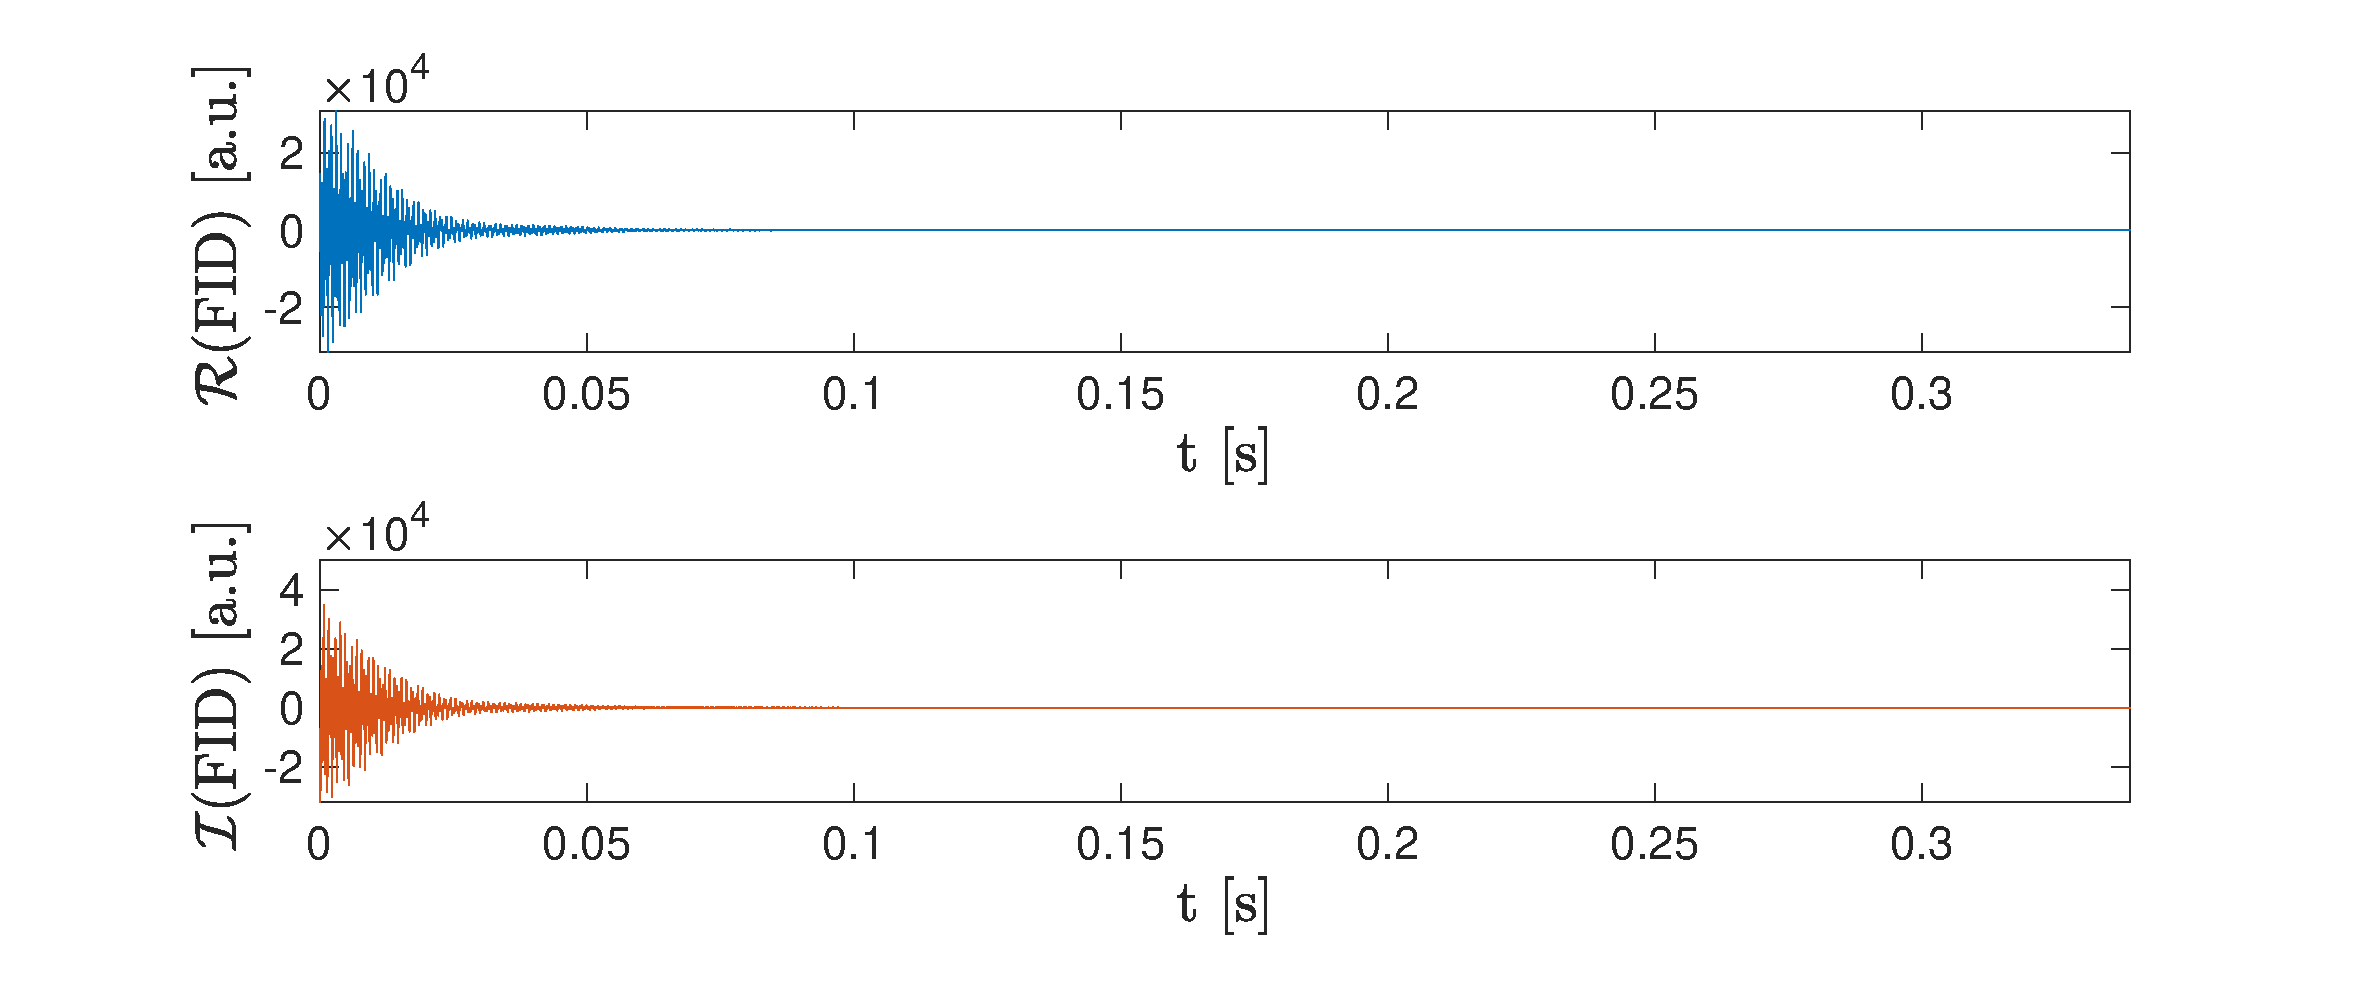
\includegraphics[width = 1.0 \textwidth]{FID.eps}
	\caption{\label{FID} Upper: plot of the real part $\mathcal{R}(FID)$ of the free-induction decay over time. Lower: plot of the imaginary part $\mathcal{I}(FID)$. }
\end{figure}  
\end{homeworkSection}

\begin{homeworkSection}{2 - Nyquist and discrete frequencies for Fourier transform}

Recall that the Nyquist-Shannon sampling theorem states that the sampling rate $\Delta t$ has to be at most $\Delta t = 1/(2f_c)$, where $f_c$ is the Nyquist frequency, for the signal to be properly reconstructed, and to avoid aliasing issues. Thus, for $\Delta t = 83.2\cdot 10^{-6}$s, one obtains that $f_c = 6.01\cdot10^{3}$Hz. The discrete frequencies spanning the interval $[-f_c, f_c]$ are then defined by $f_n := (-N/2+n)\cdot (2/N\cdot f_c)$, with $n\in\{0,…,N-1\}$.\\

\noindent Using the previously defined discrete frequencies, it is possible to discretize the chemical shift $\delta_n$ from Eq.(\ref{chemical_shift}), and changing $f$ by $f_n$. In our problem, the internal reference is taken as $f_0 = 1067.93$Hz and $\nu_0 = 800.224 \cdot 10^6$Hz.

\end{homeworkSection}

\begin{homeworkSection}{3 - Protons and chemical environment}
\begin{figure}[h!]
\centering
	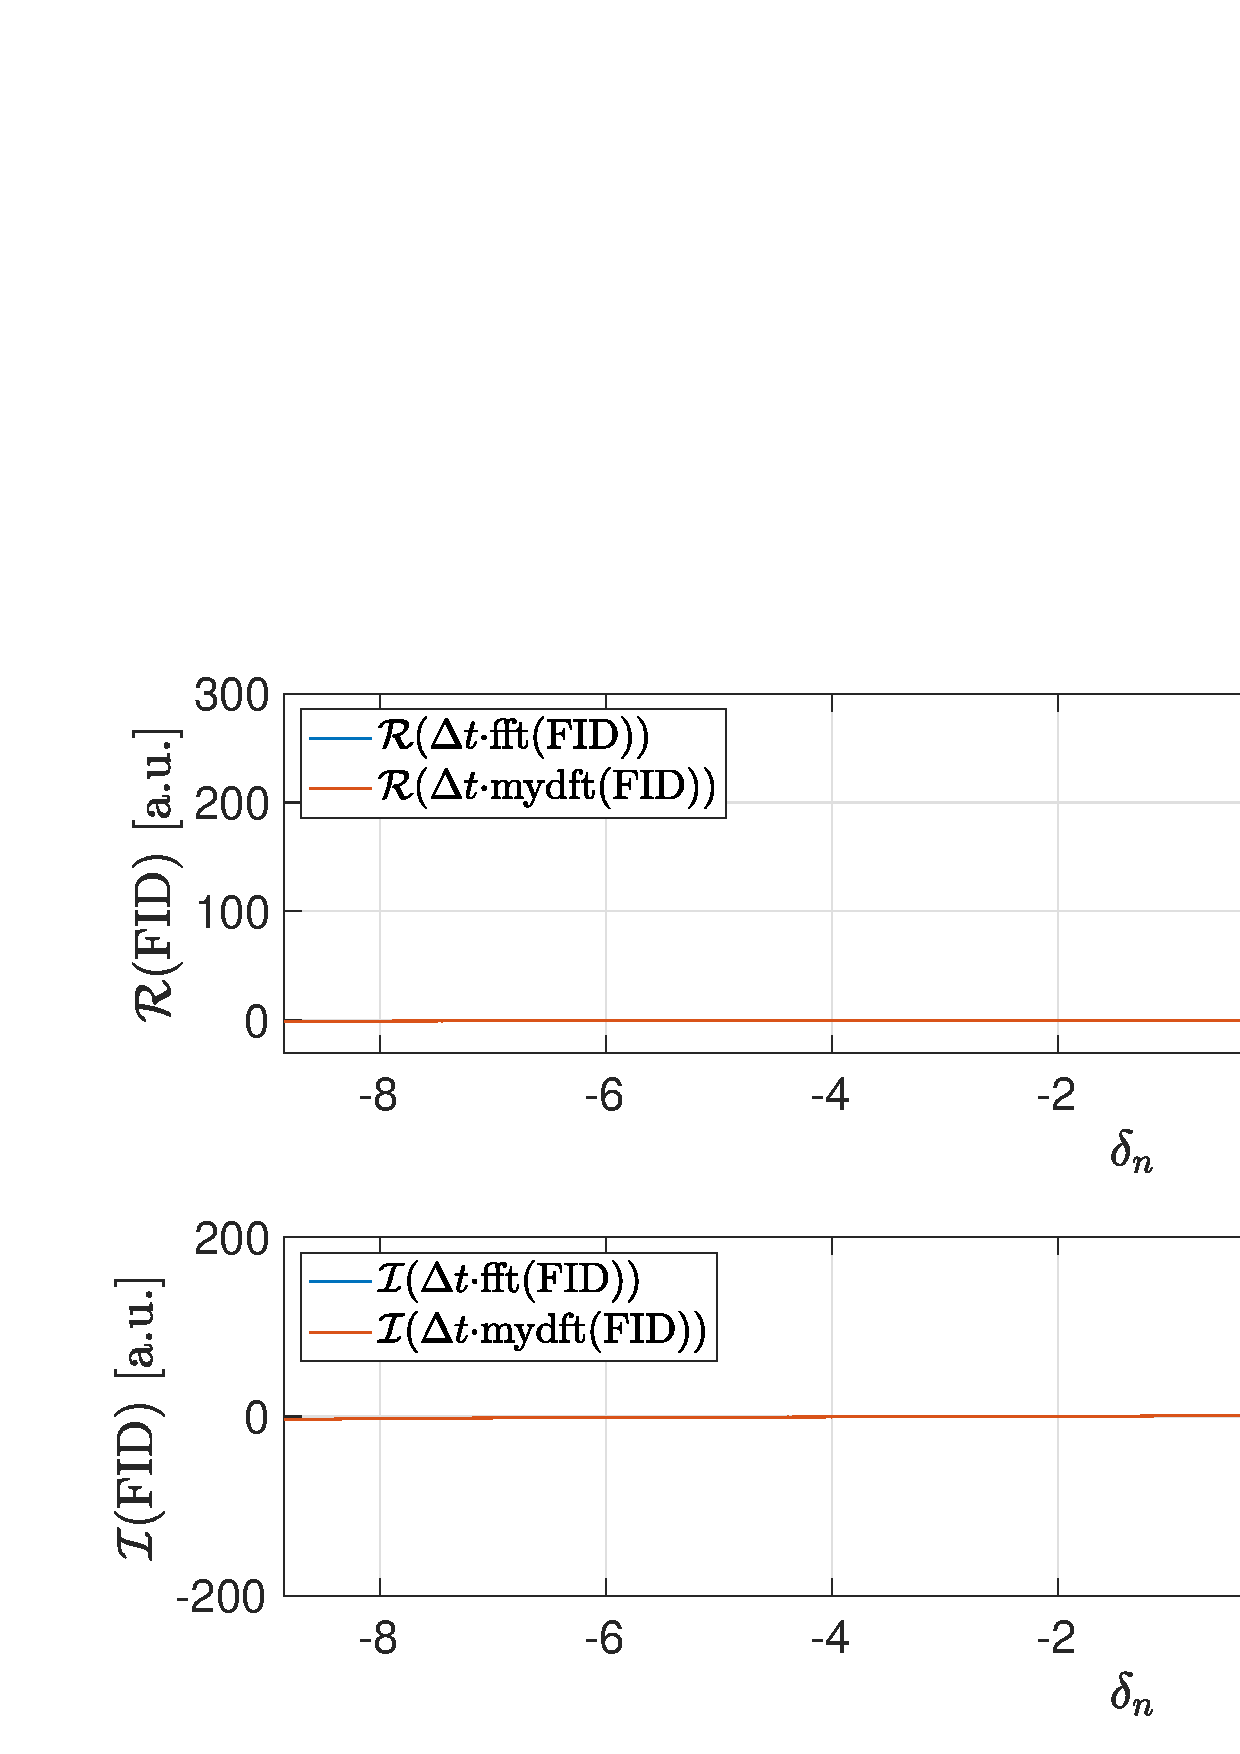
\includegraphics[width = 1.0 \textwidth]{DFT_FID.jpg}
	\caption{\label{FID_real_im} Upper: plot of the real part $\mathcal{R}(FID)$ of the free-induction decay over time. Lower: plot of the imaginary part $\mathcal{I}(FID)$. }
\end{figure}  

\noindent Fig.(\ref{FID_real_im}) shows the real and imaginary parts of the Fourier transform of the FID, as a function of the chemical shift. It displays the comparative results for both our implementation of the discrete Fourier transform \emph{mydft}, and the Matlab function \emph{fft}. Note the perfect overlap of the curves. The obtained results are identical, but the difference between the two algorithms lays in the fact that the computational complexities are not the same, and so neither are the computational times. This will be dealt with later, when introducing the \textbf{Radix-2 algorithm} for the Fast Fourier transform.\\

\noindent Fig.(\ref{power_spectrum}) shows the power spectrum of the Fourier transform of the FID as well as the relative error $\epsilon_r$ over the power spectrum between \emph{mydft} and \emph{fft}, taking \emph{fft} as the reference:\\

\beq
\epsilon_r = \Big| \frac{\text{mydft}-\text{fft}}{\text{fft}}\Big|.
\eeq\\

\noindent One notes that as said earlier, the results are identical. The error is slightly more important in the region of the peaks, and the average relative error seems to increase with $\delta$.\\

\noindent As of the chemical environment of the protons in that molecule, one notes that the upper plot from Fig.(\ref{power_spectrum}) has two very distinct peaks at $\delta_1 = 3.33$ ppm and $\delta_2 = 4.96 $ ppm respectively. Thus those two peaks are characteristics of two different chemical environment for the protons. The latter represents all the atoms the proton is related to. It is not only the particles it is chemically bonded with, but all the particles that it is close to. The area under the peaks in the power spectrum is proportional to the square of the number of protons in each environment. Since we're not able with those data only to determine the scaling law, we'll take the ratio between the two areas, both defined by\\

\beq
\mathcal{A}_i = \int_{\Omega_i} d\delta \mathcal{P}(\delta),
\eeq\\

\noindent with $\Omega_i = [\delta_i-\Delta \delta, \delta_i + \Delta \delta]$ $i=1,2$ for an appropriate $\Delta \delta$. Thus, taking the ratio $r = \mathcal{A}_1/\mathcal{A}_2$, one gets $r=1.73$. Then, there are approximately 1.73 more protons in the first chemical environment than in the second.

\begin{figure}[h!]
\centering
	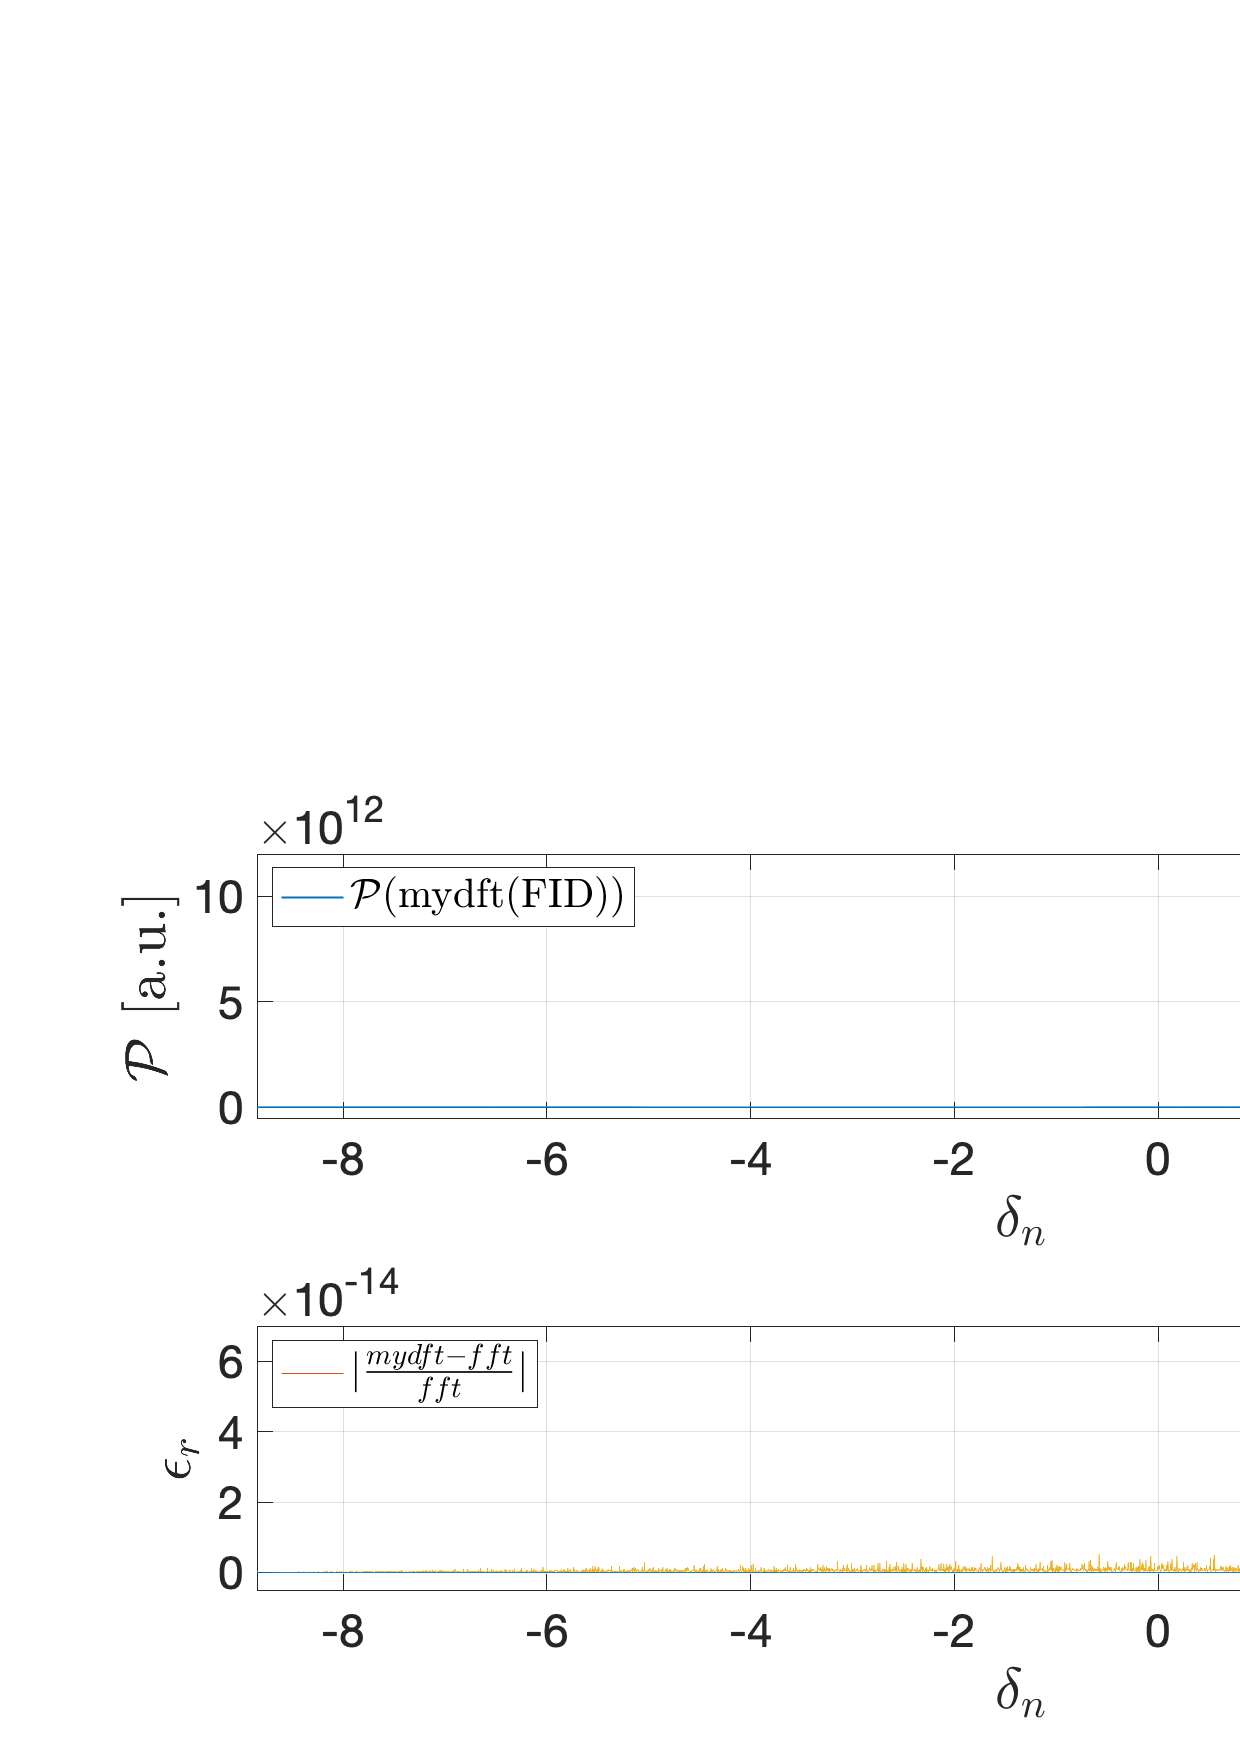
\includegraphics[width = .9 \textwidth]{Power_err.jpg}
	\caption{\label{power_spectrum} Upper: plot of the real part $\mathcal{R}(FID)$ of the free-induction decay over time. Lower: plot of the imaginary part $\mathcal{I}(FID)$. }
\end{figure}  

\noindent Considering that C, O and H atoms are able to form covalent bonds with 4, 2 and 1 neighbors respectively, it is possible to suggest the structural formula of the molecule C$_2$H$_6$O$_2$. Indeed, recall from the previous part that the molecule had two different chemical environment for protons, with about $1.73\sim2$ times more protons in one environment than the other. This means that for a molecule with 6 H atoms, equivalent to protons after forming a covalent bond, there has two be 4 H atoms with the same type of covalent bond, and 2 with a different one. Therefore, we can come up with the two following possible structures:

\begin{figure}[h!]
\centering
	\includegraphics[width = .9 \textwidth]{Comput_molecule}
	\caption{\label{molecular_struct} Two possible molecular structures for C$_2$H$_6$O$_2$}
\end{figure} 

\end{homeworkSection}
\end{homeworkProblem}

%%%%%%%%%%%%%%%%%%%%%%%%%%%%%%%%%%%%%%%%%%%%%%%%
%%%%%%%%%%%%%%%%%%%%%%%%%%%%%%%%%%%%%%%%%%%%%%%%
\newpage

\begin{homeworkProblem}

\section{Radix-2 FFT algorithm}

The discrete Fourier transform has been implemented previously in a very straightforward method. However, the computational complexity of the previous algorithm is $\mathcal{O}(n^2)$, whis is numerically very demanding. The Radix-2 Fast Fourier transform algorithm is an alternative to compute the discrete Fourier transform in $\mathcal{O}(n\log(n))$, using a recursive approach to subdivide the initial problem \cite{Yazyev}. The Matlab numerical implementation of the algorithm can be found below.\\

\begin{homeworkSection}{1- Radix-2 Fast Fourier transform algorithm} 
	\matlabscript{radix}{Matlab script for the Radix-2 Fast Fourier transform algorithm}
\end{homeworkSection}

\end{homeworkProblem}

%%%%%%%%%%%%%%%%%%%%%%%%%%%%%%%%%%%%%%%%%%%%%%%%%
%%%%%%%%%%%%%%%%%%%%%%%%%%%%%%%%%%%%%%%%%%%%%%%%%
\newpage

\begin{homeworkProblem}

\section{Fourier Ptychography}

Fourier ptychograpghy enables to overcome the problem of limited resolution in conventional optical microscopy by generating a wider aperture, that is by allowing a wider range of angles under which the light can be captured by the microscope. Indeed, denoting the resolution by $\mathcal{R}$, one gets the following relation:\\

\beq
\mathcal{R} \propto \frac{\lambda}{n \sin(\theta)},
\eeq\\

\noindent where $\lambda$ is the wavelength of the incoming light, $n$ the refractive index of the lens and $\theta$ the maximum angle of acceptance. It is then trivial that increasing $\theta$ will increase $\mathcal{R}$.\\

\noindent In order to understand the Fourier ptychography algorithm, let us recall how a typical optical microscope works. Considering that the studied object can be represented by a 2-dimensional complex function $O$, that is the real space image is given by $O(x,y)$, where $(x,y)$ is an appropriate coordinate choice. Thus, the reciprocal (Fourier space) image is given by $\mathcal{F}(O)(k_x,k_y)\cdot a(k_x,k_y)$, where $\mathcal{F}$ represents the Fourier transform operator and $a$ an amplitude transfer function of finite radius. The latter can be approximated by a low-pass filter of radius $r_c$, mapping to $1$ below $r_{c}$ and $0$ otherwise. The real image is then reconstructed after the light passes through the second lens, and the detector will record an intensity $I \propto |\mathcal{F}^{-1}\Big(\mathcal{F}(O)(k_x,k_y)\cdot a(k_x,k_y)\Big)|^2$.\\

\noindent In Fourier ptychography, the process is slightly different since instead of using perpendicular plane waves $\propto e^{ik_{zi}z}$ as illumination sources, several images are taken with tilted light sources $\propto e^{ik_{xi}x}e^{ik_{yi}y}e^{ik_{zi}z}$. Then the Fourier transform is shifted as follows:\\

\beq
\mathcal{F}(O)(k_x-k_{xi},k_y-k_{yi}),
\eeq\\

\noindent and hence, the intensity recorded by the microscope verifies\\

\beq
I \propto \Big|\mathcal{F}^{-1}\Big(\mathcal{F}(O)(k_x-k_{xi},k_y-k_{yi})\cdot a(k_x,k_y)\Big)\Big|^2.
\eeq\\

\noindent The cutoff circle has then been shifted by $(k_{xi}, k_{yi})$ and some higher frequencies were involved in the image formed. Thus, taking several images under tilting angles enables to reconstruct the Fourier transform with a higher cutoff radius, and enhance the resolution.\\

\subsection{Numerical implementation of Fourier ptychography algorithm}
\vspace{1cm}

In the next part, the following reconstruction algorithm will be used \cite{Yazyev}:\\

\noindent 
\newpage
\begin{enumerate}
\item{Start with a (complex) guess function $I$ and compute $\mathcal{F}(I)$.}
\item{Restrict $\mathcal{F}(I)$ to a circle in Fourier space, centered around $(k_{xi}, k_{yi})$ multiplying it by a cutting function: $\mathcal{F}(I)\rightarrow \mathcal{F}(I)_c =\mathcal{F}(I)\cdot C_{(k_{xi}, k_{yi})}$}
\item{Take its inverse Fourier transform $\mathcal{F}^{-1}(\mathcal{F}(I)_c)$}
\item{Retain the phase but replace the magnitude by the experimental one}
\item{Perform the Fourier transform of the resulting object and use it to replace the values of $\mathcal{F}(I)$ inside the cutoff circle}
\item{Repeat the previous steps for the the circles in Fourier space, that is for different values of $(k_{xi}, k_{yi})$}
\item{Repeat the previous algorithm till convergence is reached}
\end{enumerate}


\begin{homeworkSection}{1 - Phase and Intensity}
\begin{figure}[h!]
\centering
	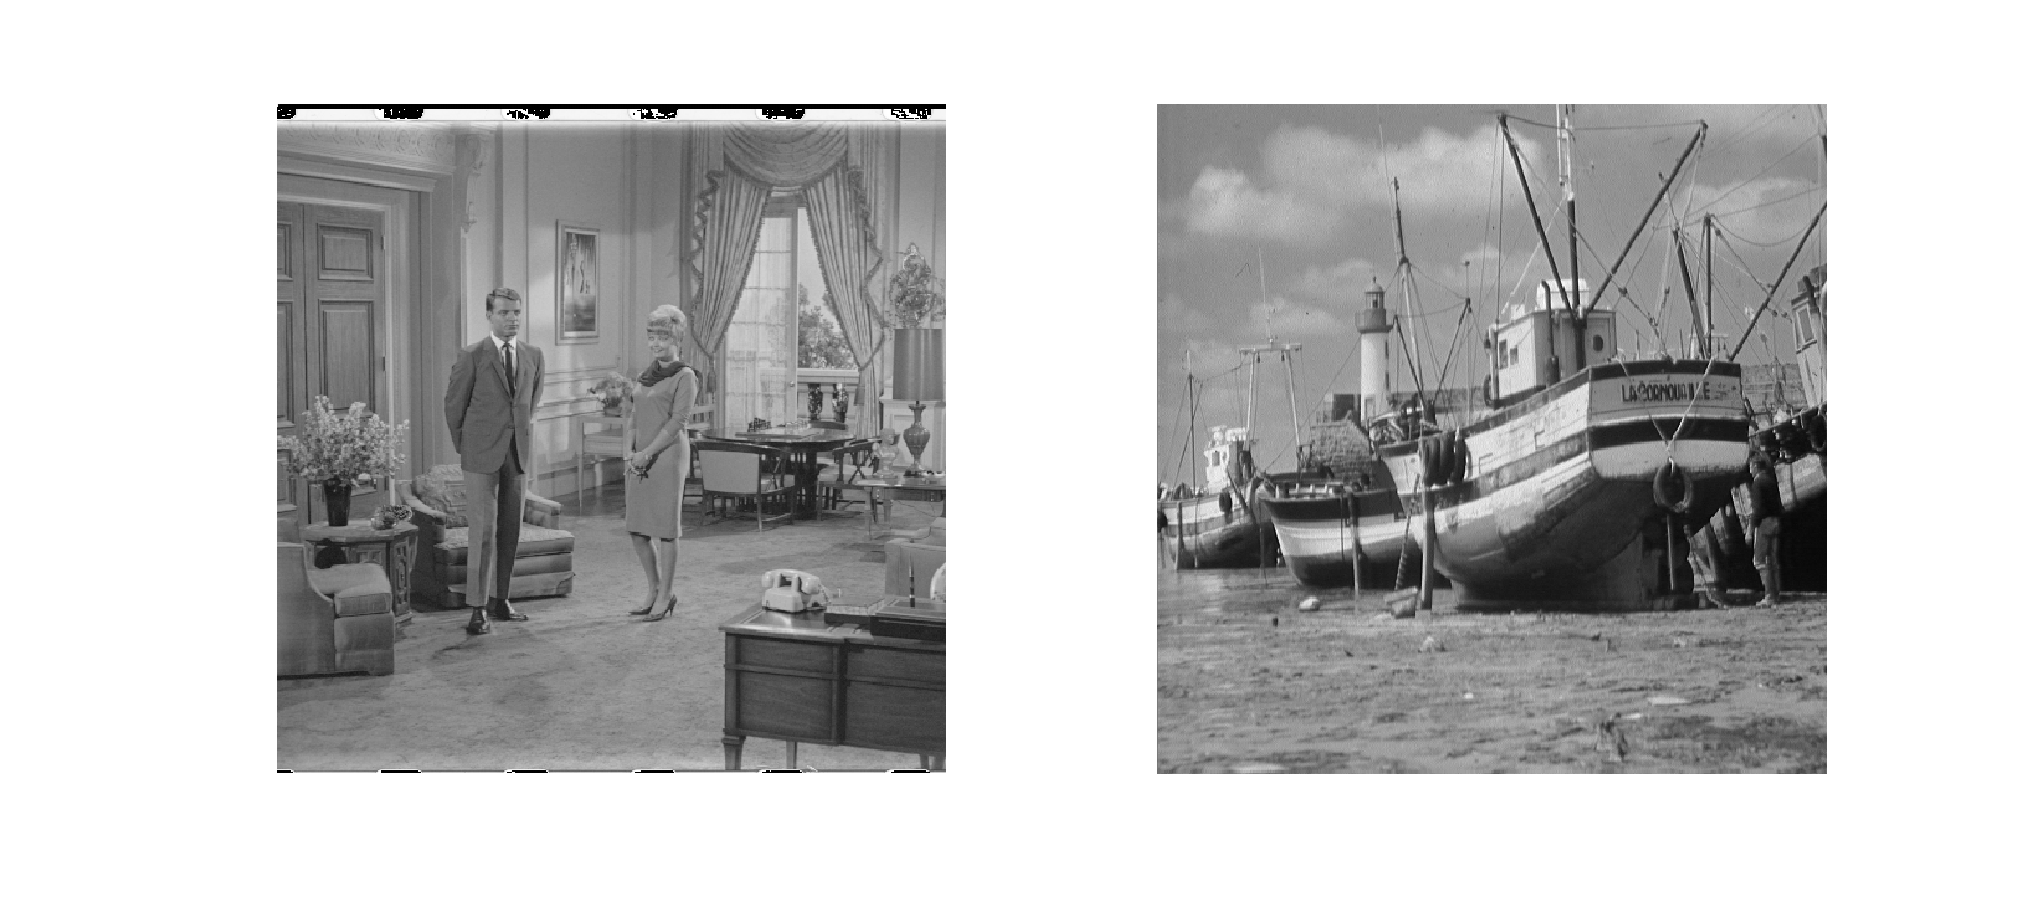
\includegraphics[width = .9 \textwidth]{phase+intens.eps}
	\caption{\label{phase_intens} Left: Original intensity image - Right: Original phase image }
\end{figure} 

\noindent Fig.(\ref{phase_intens}) displays both the original intensity and the original phase. By mean of Fourier ptychography, on some simulated microscope images, we will try to retrieve the phase and enhance the resolution. The implementation of the above algorithm will be described and the results will be presented below. 

\end{homeworkSection}

\begin{homeworkSection}{2 - Microscope images}
The microscope images were obtained by taking the Fourier transform of the original objects, and by applying circular filters in Fourier space, before taking the inverse Fourier transform and record the new intensity. Fig.(\ref{microscope}) shows an example of such a 'microscope' image. One notes that the result obtained in Fourier space is not contained in the original circular low pass filter. This is due to the fact that when  


\begin{figure}[h!]
\centering
	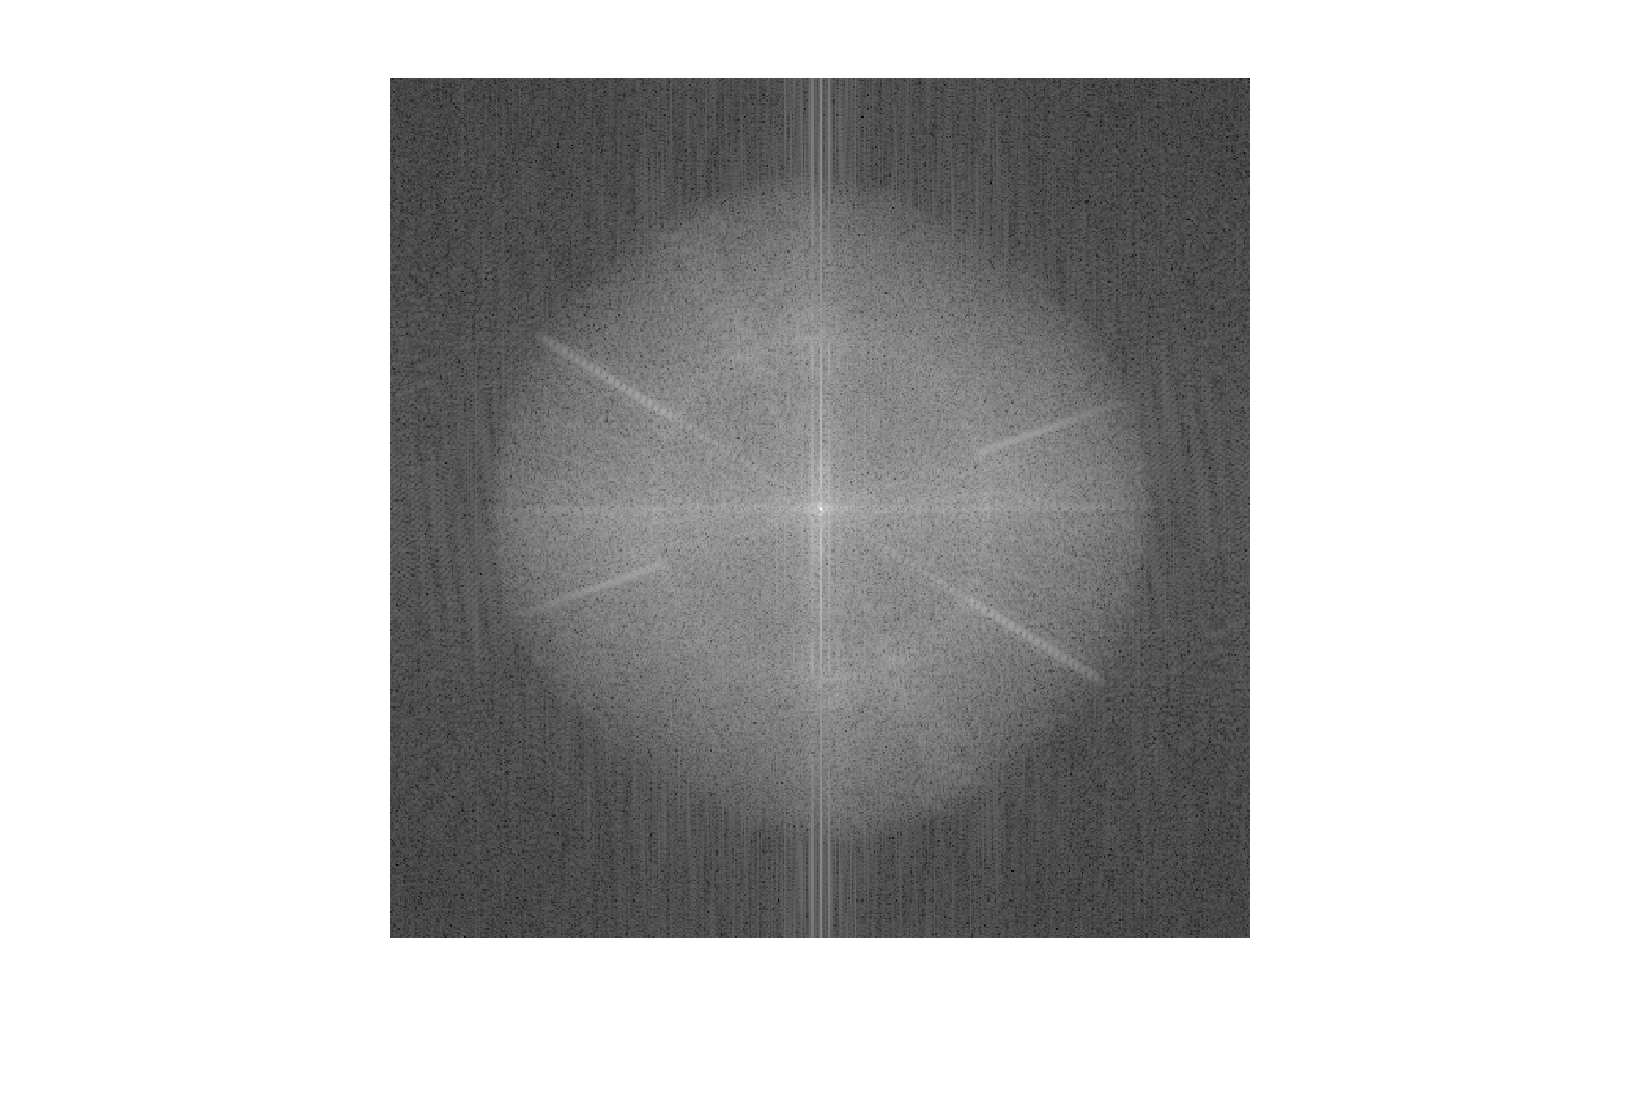
\includegraphics[width = .5 \textwidth]{ptychography00.eps}
	\caption{\label{microscope}  Fourier transform of the image ptychography00.png }
\end{figure} 
\end{homeworkSection}


\begin{homeworkSection}{3 - Algorithm and filter}
Let us take for initial guess the unit function $I(x,y) = 1$ $\forall x,y$ on the grid. Performing the Fourier transform on that constant function will yield a Dirac Delta function in Fourier space, hence the pixel on the left plot of Fig.(\ref{filter_fig}). Restraining the Fourier transform by mean of a fixed aperture (cutoff disk) centered at the center of the grid (see middle plot on Fig.(\ref{filter_fig})) will not affect the pixel since it is inside the 'passing region' of the filter. The right plot of Fig.(\ref{filter_fig}) indeed confirms that remark. 


\begin{figure}[h!]
\centering
	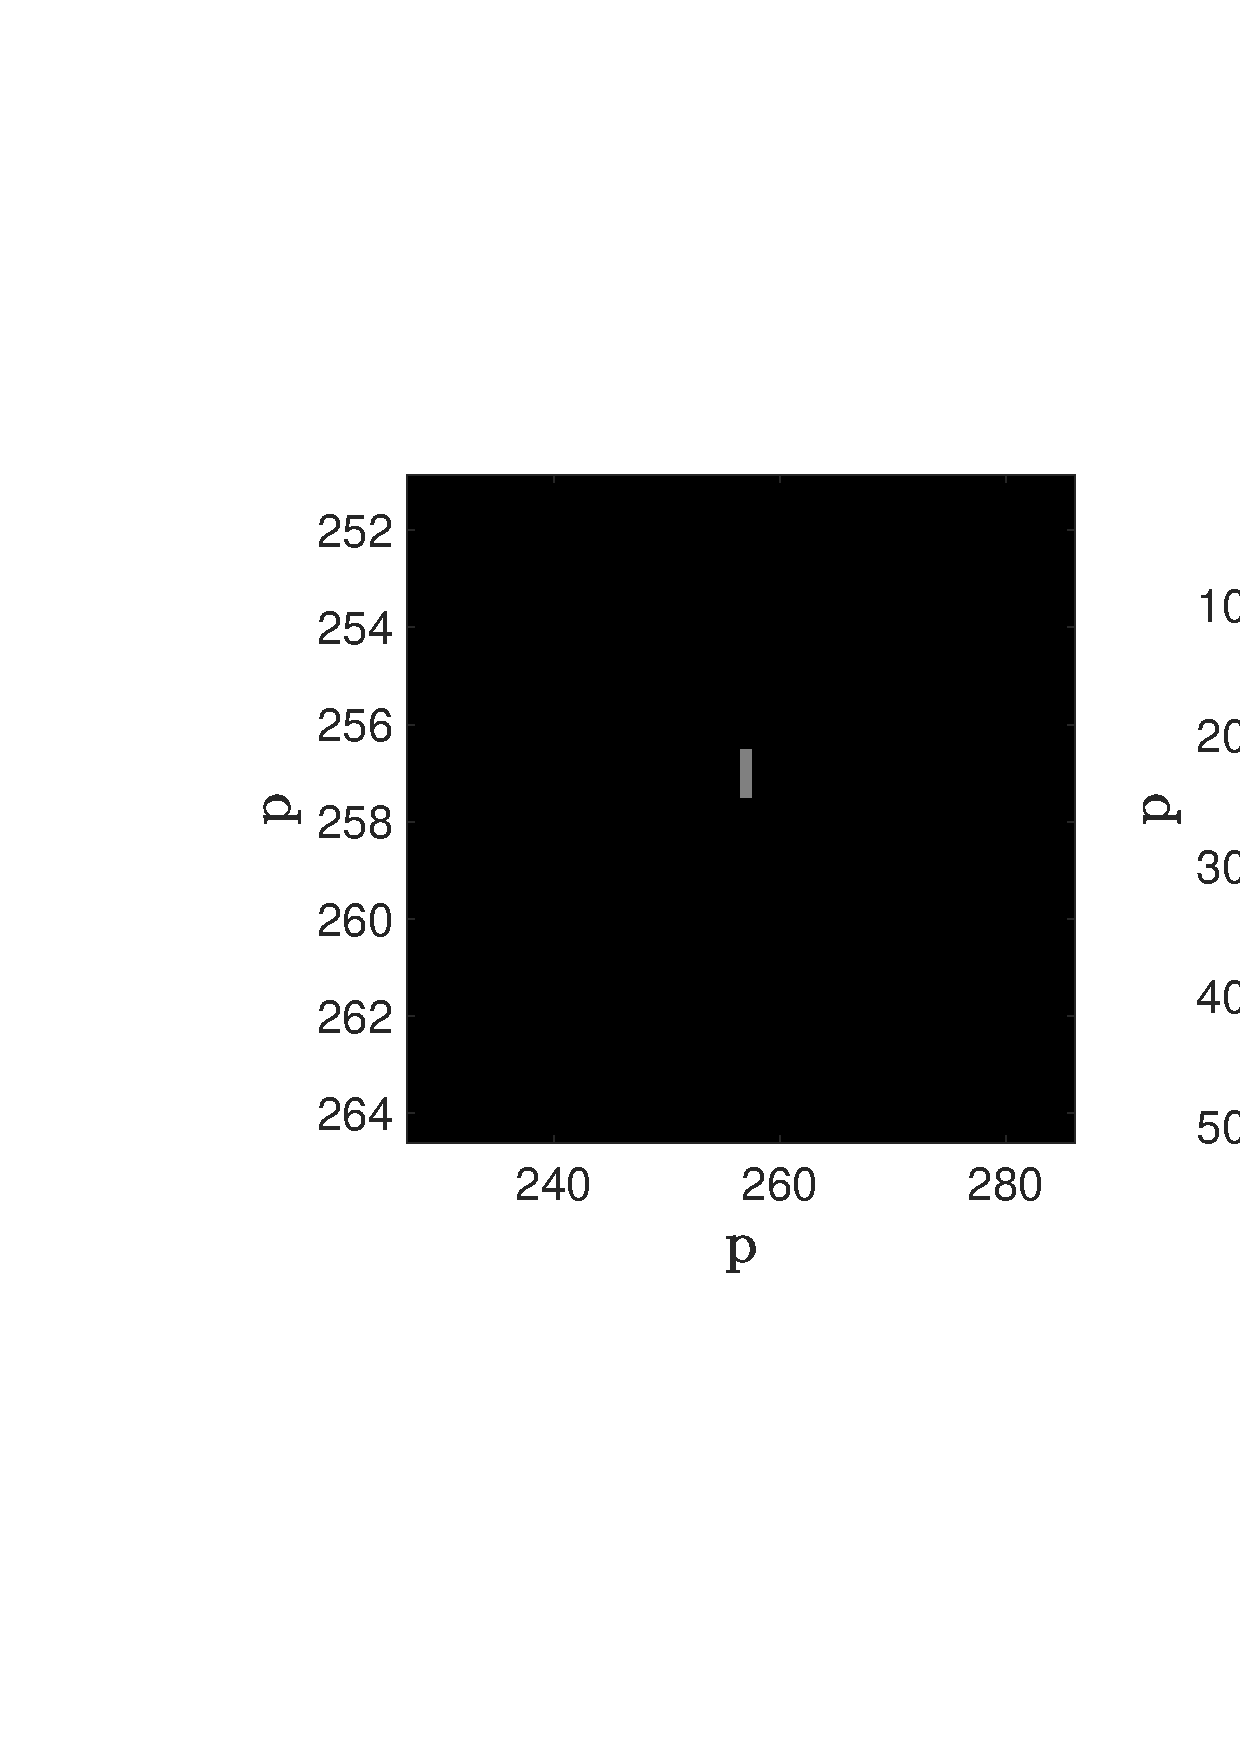
\includegraphics[width = 1 \textwidth]{filter.pdf}
	\caption{\label{filter_fig}  Left: Fourier transform of constant unit guess. Middle: Cutoff filter for constrained aperture in Fourier space. Right: Result after applying the filter to the left image.}
\end{figure} 
\end{homeworkSection}

\begin{homeworkSection}{4 - Guess improvement }

The initial guess can be improved by taking the inverse Fourier transform of the previous result, keeping the phase and replacing the intensity by the one measured on the image \emph{ptychography00.png}. Fig.(\ref{guess_updated}) illustrates the concept of phase retrieval through the application of this procedure. Indeed, a comparison between Fig.(\ref{microscope}) and Fig(\ref{guess_updated}) confirms that. \\
 
\begin{figure}[h!]
\centering
	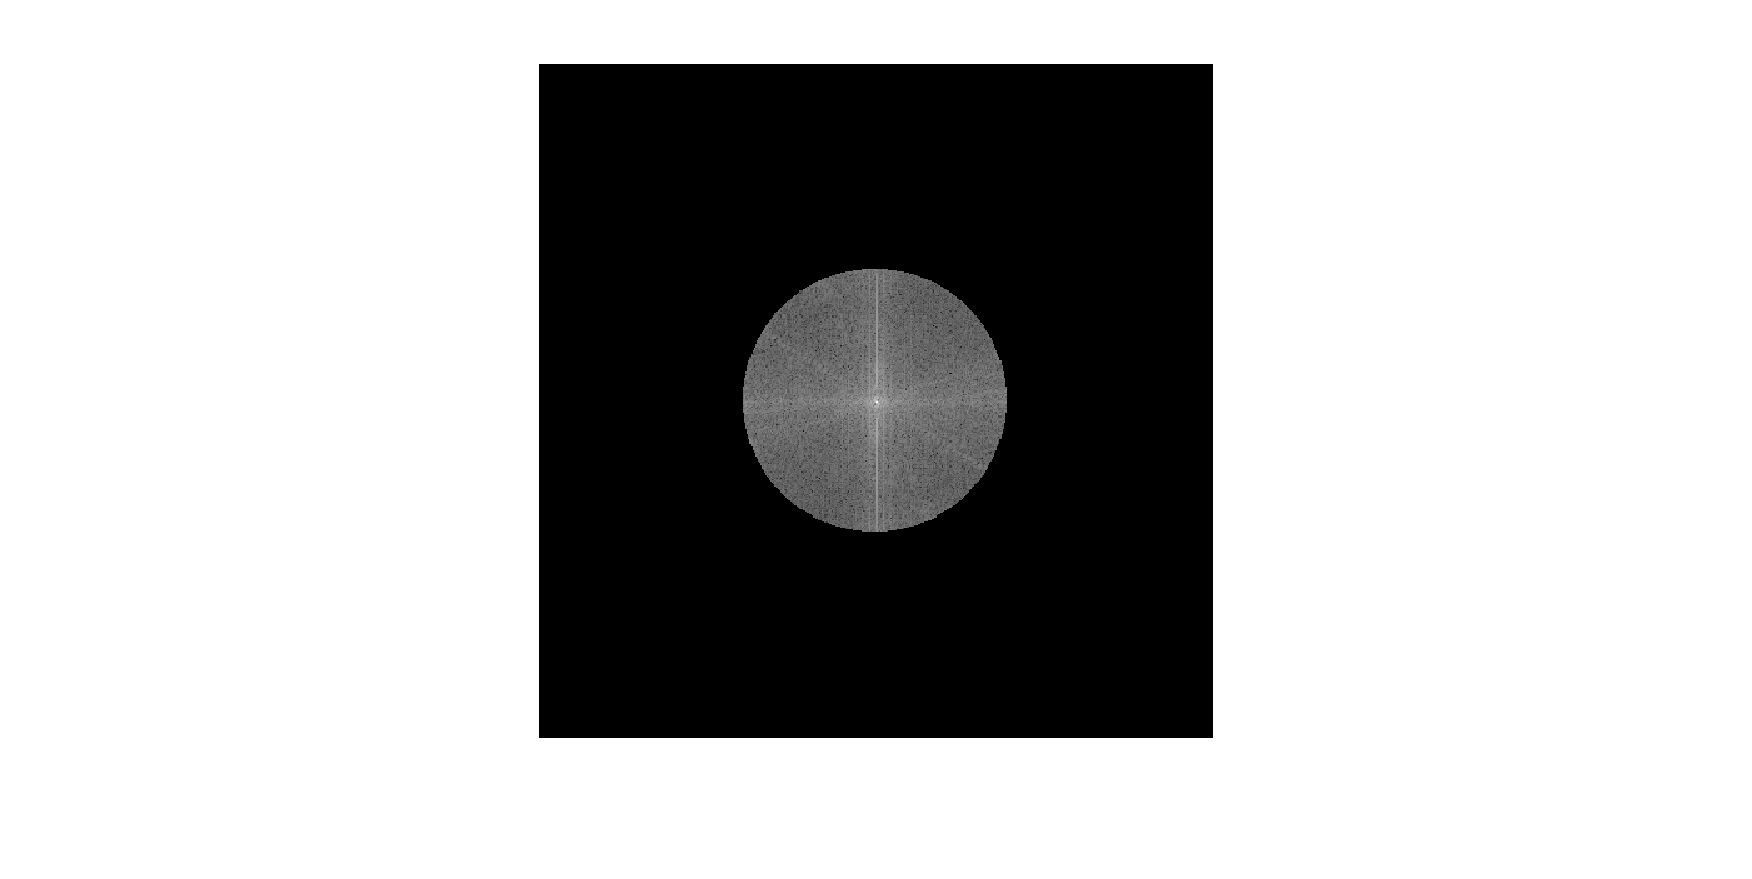
\includegraphics[width = 0.7 \textwidth]{guess_updated.eps}
	\caption{\label{guess_updated} Phase retrieval process illustration. The Fourier transform of the initial guess is represented, with the intensity from \emph{ptychography00.png}}
\end{figure} 
\end{homeworkSection}


\begin{homeworkSection}{5 - One iteration}
The previous guess can be further improved by combining guesses all the 'microscope images' \emph{ptychography-i,j.png}. The cutoff filter is shifted on the grid for each of them and the cutouts are combined to form a better guess of the Fourier transform of the initial object. Fig.(\ref{one_step}) demonstrates that, representing on the left the intensity and on the right the phase of the inverse Fourier transform of that combined and improved guess. The similarity with the initial images from Fig.(\ref{phase_intens}) is quite obvious.\\

\begin{figure}[h!]
\centering
	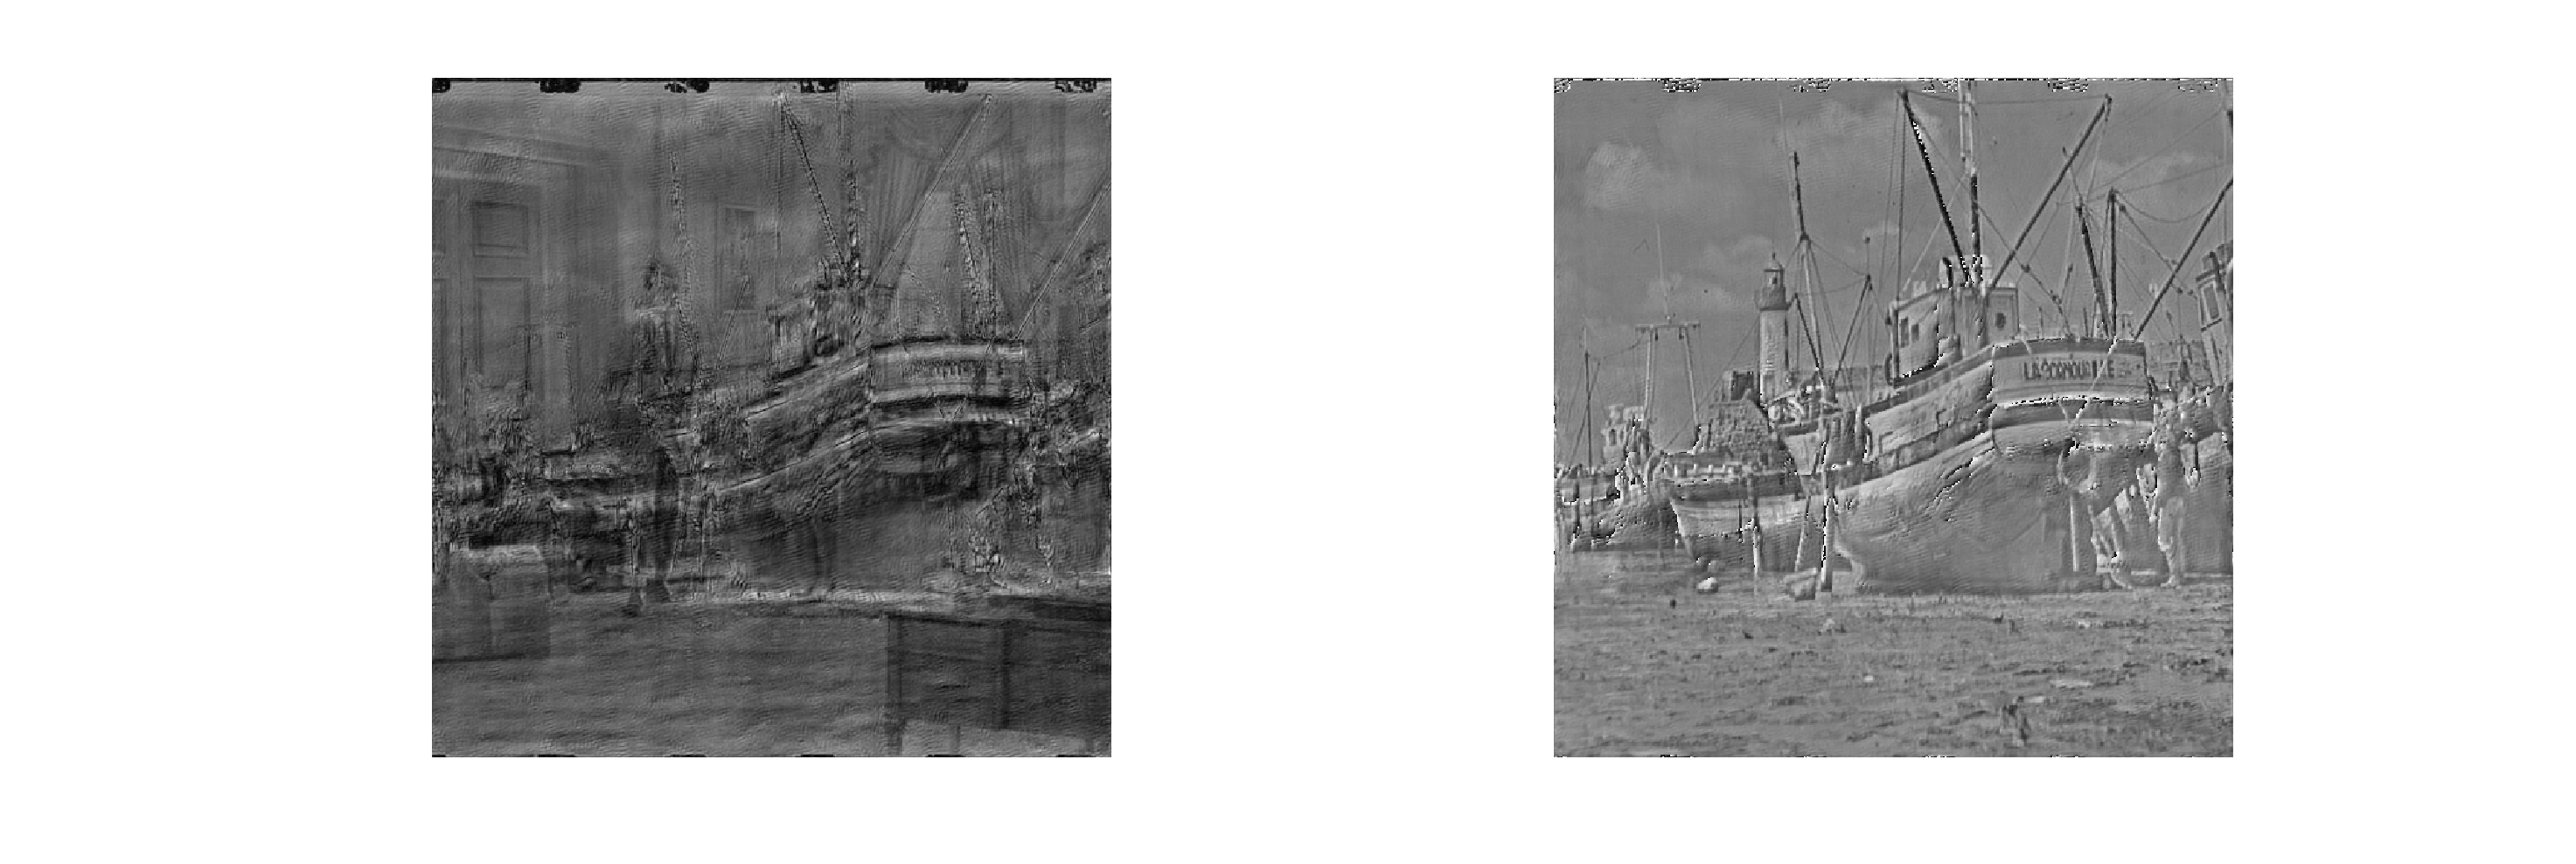
\includegraphics[width = 1 \textwidth]{one_step.eps}
	\caption{\label{one_step} Left: Intensity from the inverse Fourier transform of the improved guess. Right: Phase for the same. }
\end{figure} 
\end{homeworkSection}

\begin{homeworkSection}{6 - Iterative process}

The process described above can be repeated a certain amount of times, typically till convergence occurs. However, in our case, we will limit to 20 iterations, and not test for convergence. Fig.(\ref{final_ptycho}) displays the results for the intensity and for the phase after 20 iterations of the previous algorithm. Note that the the images are much more focused than after one iteration. However, the result is still a little blurry compared to the initial images from Fig.(\ref{phase_intens}).

\begin{figure}[h!]
\centering
	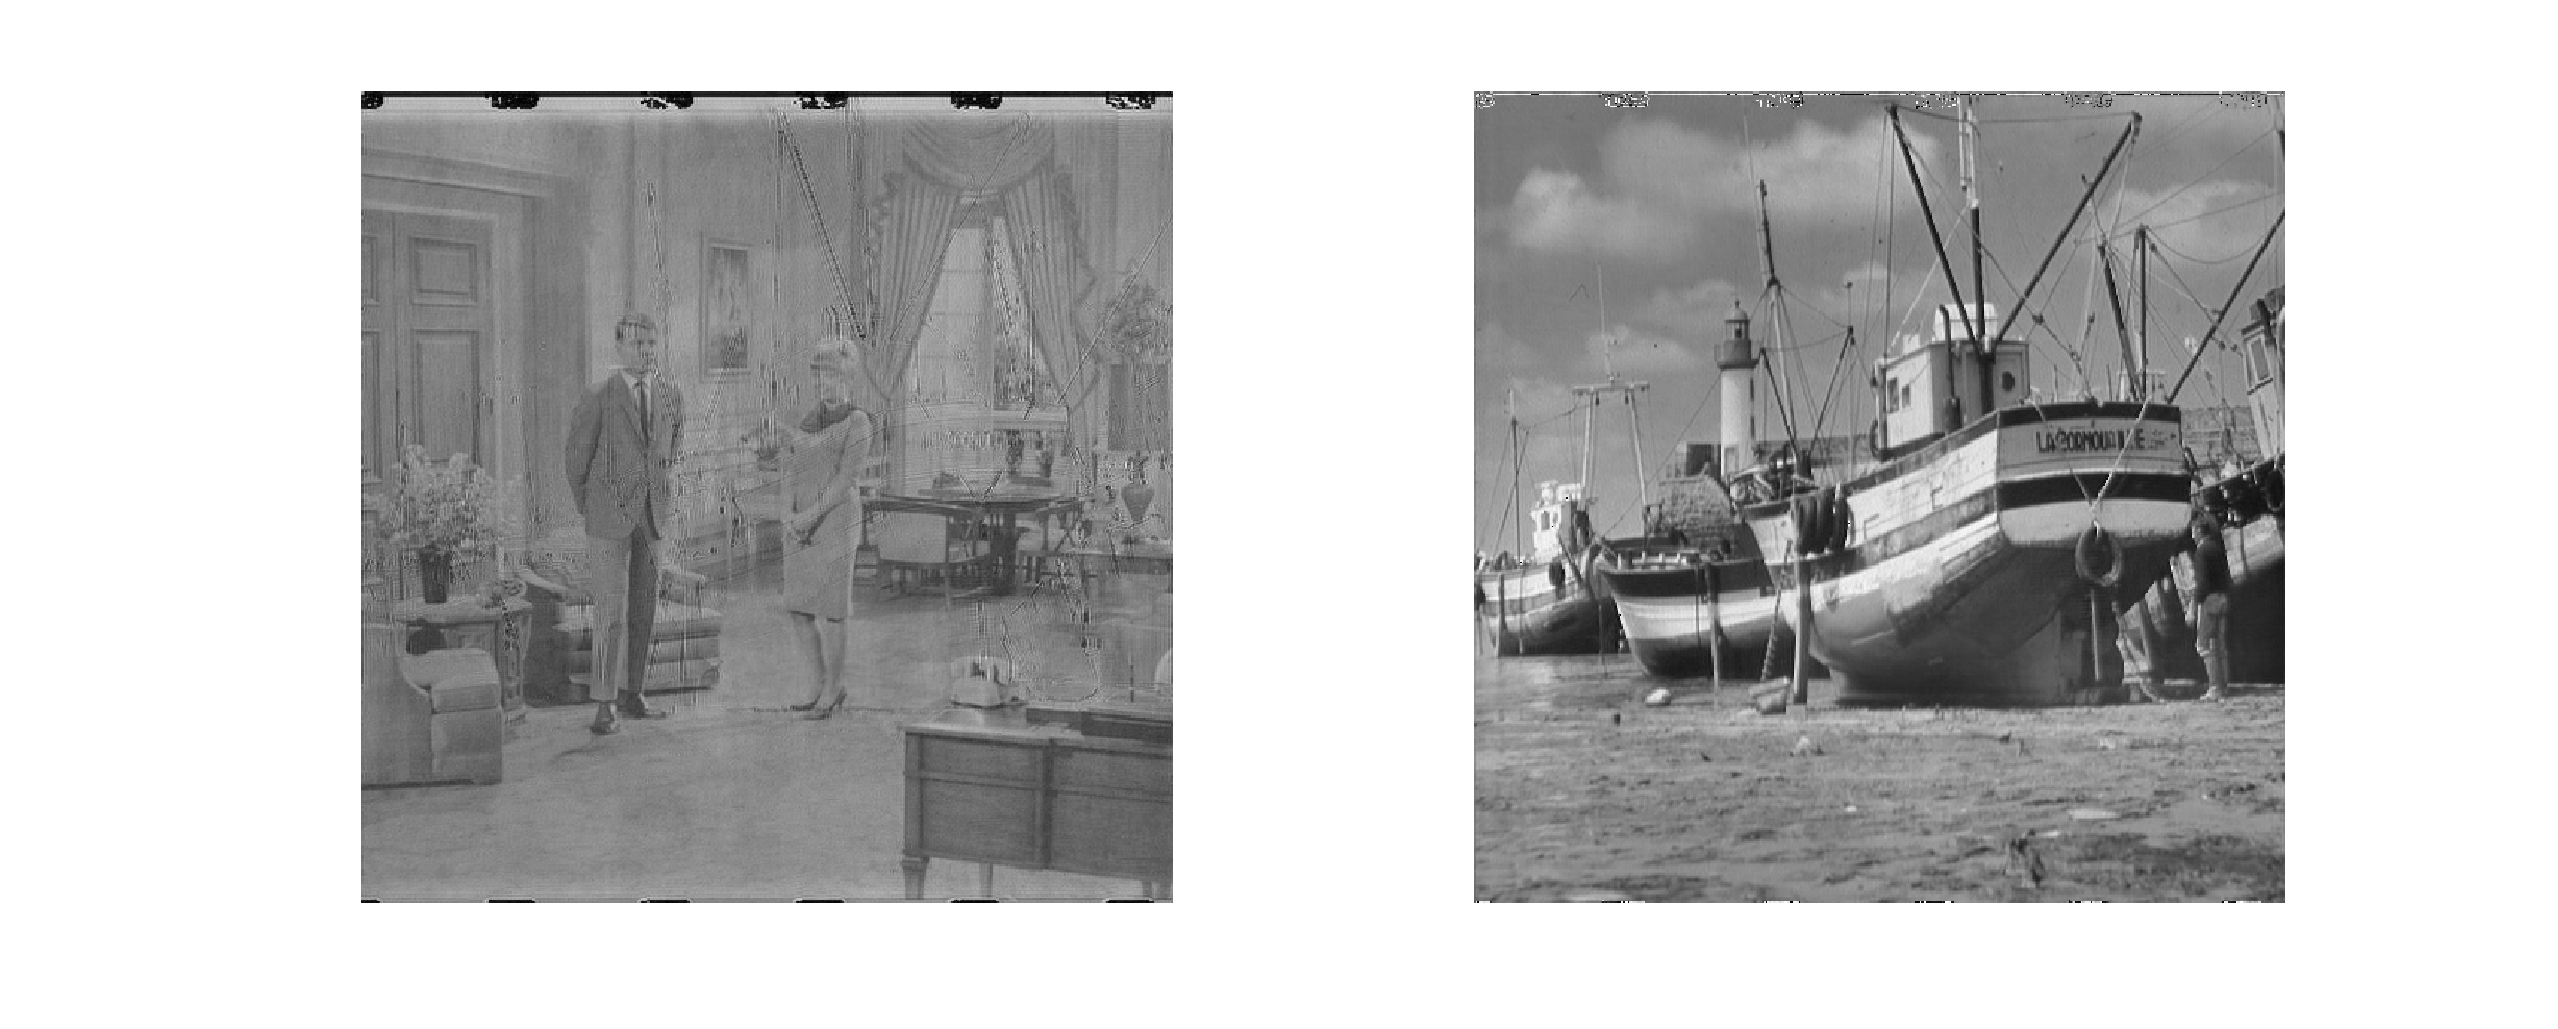
\includegraphics[width = 1 \textwidth]{final_ptycho.eps}
	\caption{\label{final_ptycho}  Left: Intensity after 20 iteration of the Fourier Ptychography algorithm. Right: Same for the phase.}
\end{figure} 
\end{homeworkSection}



\end{homeworkProblem}


\end{spacing}

\newpage
\bibliographystyle{alpha}
\bibliography{references}
\end{document}
\end{document}

%%%%%%%%%%%%%%%%%%%%%%%%%%%%%%%%%%%%%%%%%%%%%%%%%%%%%%%%%%%%%
